\documentclass[a4paper, 11pt]{article}
\usepackage[a4paper,bindingoffset=0.2in,%
            left=0.3in,right=0.4in,top=1in,bottom=1in,%
            footskip=.25in]{geometry}
\usepackage{graphicx}
\usepackage{subcaption}
%	options include 12pt or 11pt or 10pt
%	classes include article, report, book, letter, thesis

\title{\vspace{-3cm}%
  Fundamentals of Data Science - Final Project \\
  \large }
\author{Andrea Formichetti ID-1764939}
\date{09 February 2017}
\begin{document}
\maketitle

In this challenge we are being asked to produce a prediction about sale prices of residential homes in Ames, Iowa. Train set and  test set needed for the prediction is provided as two separated CSV file, we want to produce another CSV file containing for each row the Id of the house and a prediction for the sale price. Follow the procedure adopted.

\section{Preprocessing}
In this part I tried to wipe the dataset as much as possibile in order to make our predictions more accurate.
\paragraph{Make trainset bigger}
Cutting off price column from the trainset and merge the two datasets together result in a larger dataset and hopefully in a better estimation.
\paragraph{Drop features with too many missing values}
I drop all features that have more than 40\%(empirically chosen) of missing values(NA) among its entries. This features are too much uninformative and it would ruin the regression.
\paragraph{Remove outliers} 
In this phase I remove from the trainset all entries identified as outliers, in particular all those that after normalization exceed the standard deviation more than 5 times. That's because linear models are quite sensible to the outliers. 
\paragraph{Compute the skewness and take the Log}
I detect the features that has an high skewness and I transform it taking $log(feature + 1)$ in some sense it make the feature more "Normal".
\paragraph{Generate dummy variables}
A lot of features among the 79 that compose the dataset are categorical, which is it take value from a finite list of string representing some quality, we need to convert it to something that can be inserted in our model. Generate a boolean variable for each possible value is a way, in this case work well.
\paragraph{Substitute missing values with the mean}
Here I sobstitute all the remaining missing values with the mean of the respective feature, this actually allows to compute regression even with points that include some NaN and at the same time avoids to introduce distorsions. 

\section{Model Selection}
In this part I evaluate which model to use for computing the regression. Essentialy I tried three different linear models: \textbf{Linear Regression}, \textbf{Ridge Regression} and \textbf{Lasso regressio}n. For each model attempts have been made to modify a bit the parameters defined into Preprocessing part to "adapt", as far as possibile, the dataset to  the model in use (for example the threshold that define the condition of being  an outlier)
\paragraph{Cross Validation}
In the train phase I iteratively use the cross validation tecnique to evaluate the model in use and to find, when needed, the optimum parameter for them ($\alpha$ for Ridge and Lasso). In the next page there will be some explanatory images.
\\ \\
The model that has produced better results is Lasso with a kaggle-score(\emph{RMSE} between log of predictions and observed value) of \textbf{0.11892}. In the next page there's an image that show residual of the prediction on the trainset, it looks pretty good! 
\\Further details can be found in comments of the python script.

\begin{figure}[t]
\caption{Plot of $R^2$ with respect of $\alpha$ obtained into cross validation of \textbf{Lasso} model, best $R^2 = 0.9244$}
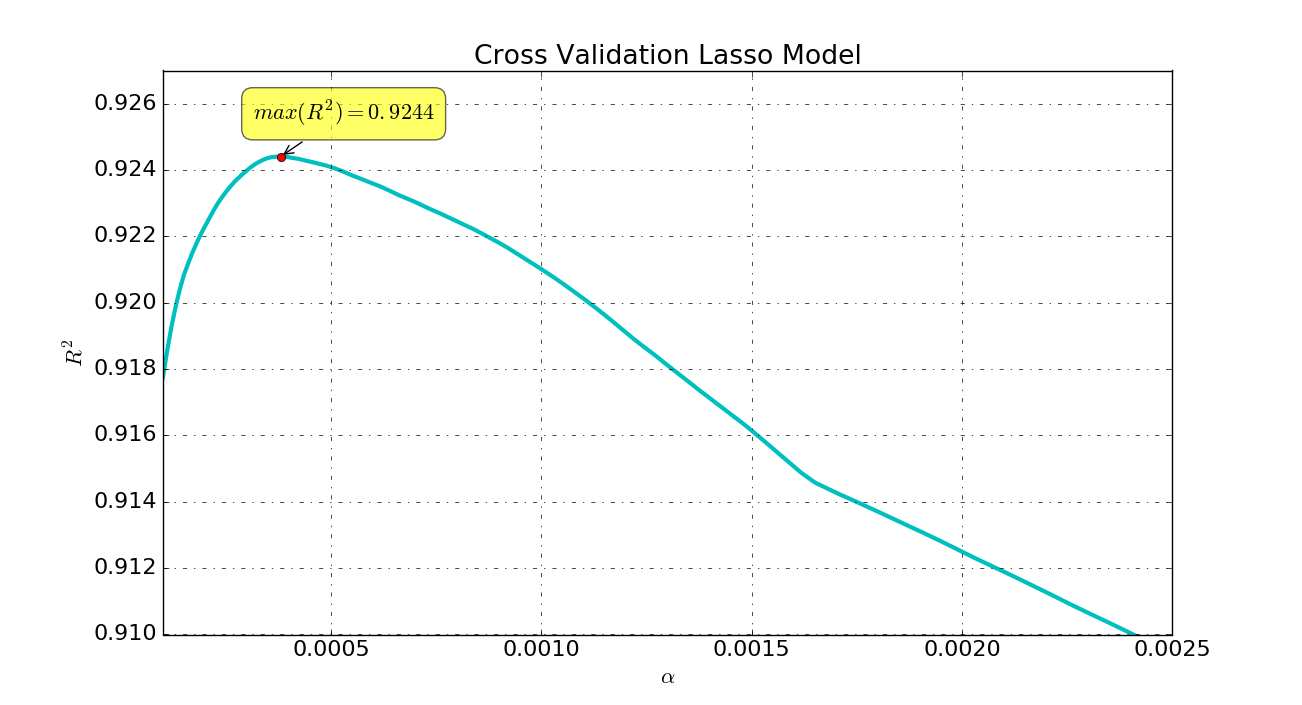
\includegraphics[width=20cm]{r2lasso.png}
\centering
\end{figure}

\begin{figure}
\centering
\begin{subfigure}[b]{10cm}            
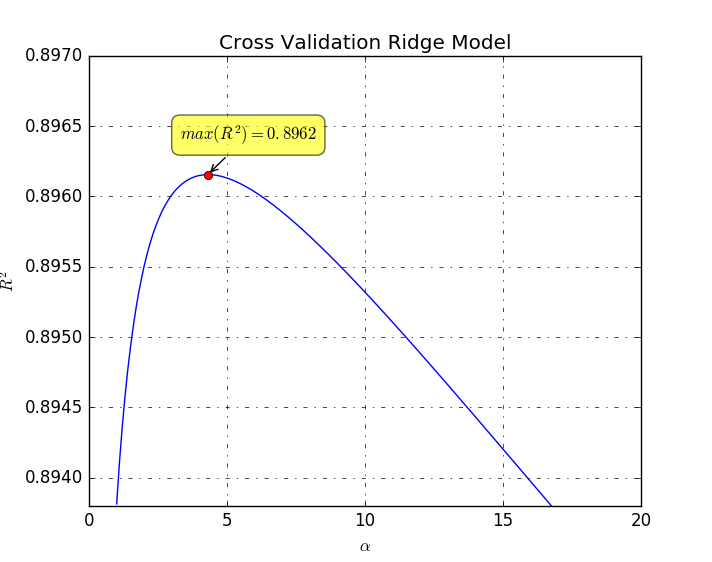
\includegraphics[width=10cm]{r2ridge.png}
\caption{Plot of $R^2$ with respect of $\alpha$ obtained into cross validation of \textbf{Ridge} model,best $R^2 = 0.8962$}
\label{Fig:Data1}
\end{subfigure}
\begin{subfigure}[b]{8cm}
\centering
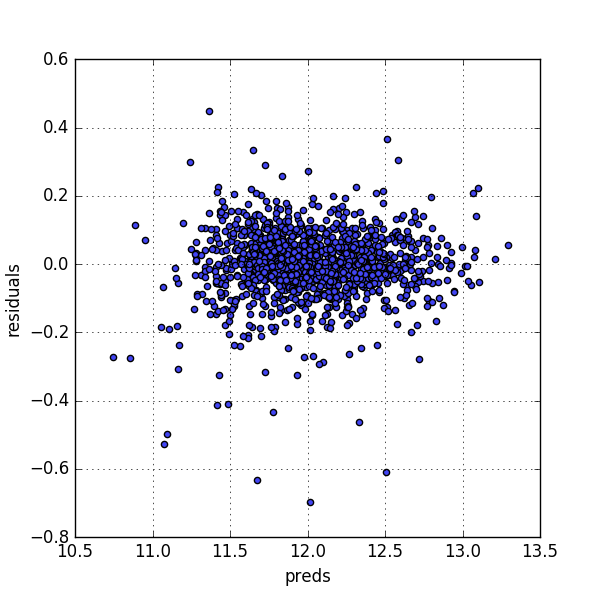
\includegraphics[width=8cm]{residuals.png}
\caption{Plot of residuals obtained from \textbf{Lasso} regression on the trainset}
\label{Fig:Data2}
\end{subfigure}
\label{fig:TOF}
\end{figure}

\end{document}

